\documentclass[12pt]{article}
\usepackage{graphicx}
\usepackage[utf8]{inputenc}
\usepackage{amsmath}
\usepackage{float}
\usepackage[top=20mm,bottom=21mm,left = 30mm , right = 30mm]{geometry}
\usepackage{xcolor}
\usepackage{wrapfig}
\usepackage{caption,subcaption}
\usepackage{hyperref}
\hypersetup{colorlinks,
citecolor=black, filecolor=black, linkcolor=black, urlcolor=black}
\usepackage{setspace}
\usepackage{pdfpages}
\usepackage{cite}

\title{Autocorrelation in Weather}
\author{Matthew Campos}
\date{October 22, 2019}
\begin{document}
    \maketitle

    \section{Introduction}
    The purpose of this analysis is to answer the question:  Are temperatures of one year significantly correlated with the next year (successive years), across years in Key West, Florida? The script written is to calculate the correlation of n-1 pairs of years, where n is the total number of years. In order to have a sufficient amount of data for meaningful analysis, random sampling was utilised on the data. The data collected from KeyWestAnnualMeanTemperature.Rdata, consists of temperature recordings in the 20th century, from 1901 to 2000. Thus the correlation calculated was 100 years of data, sampled to simulate different temperature possibilities.

    \section{Method}
    To simulate different sets of data, a script was written that randomly sampling the original data 10,000 times. This was written using a for loop to create 10,000 samples, and the sample() function in RStudio, to randmoly select 100 different data points each sample, from the original data. To calculate the correlation of pairs of years, two vectors were created. The first contained the values of the first 99 data points, excluding the 100th data point, while the second vector excluded the first data point.The script would then calculate the correlation of both vectors storing the result in a results vector. This was repeated 10,000 times. Finally, an equation to calculate p-value was written to see if the correlation was significant. Since the measurements are not indepedent, cannot use the standard p-value.

    \section{Result}
    The figure below shows the frequency of calculated correlation coefficient values from the simulation, in blue. We can see that follows the shape of a random distribution. The black line is the correlation value of the original dataset. A vaue of 0.3261697 suggests that there is a very slight positive correlation of data. The random distribution shows that frequency of the correlation coefficients occuring by chance. Since the value of original correlation falls tends towards the right tail end of the distribution, it is significant. This is supported with the p-value. A p-value of 0.0001 is less than the alpha value, 0.05. Therefore, the null hypothesis can be rejected and there is a correlation in temperatures of successive years.

    \begin{figure}[t!]
        \caption{Histogram showing 10,000 simulation of weather data correlation values. Original data correlation = 0.3261697, P-value = 0.0001}
            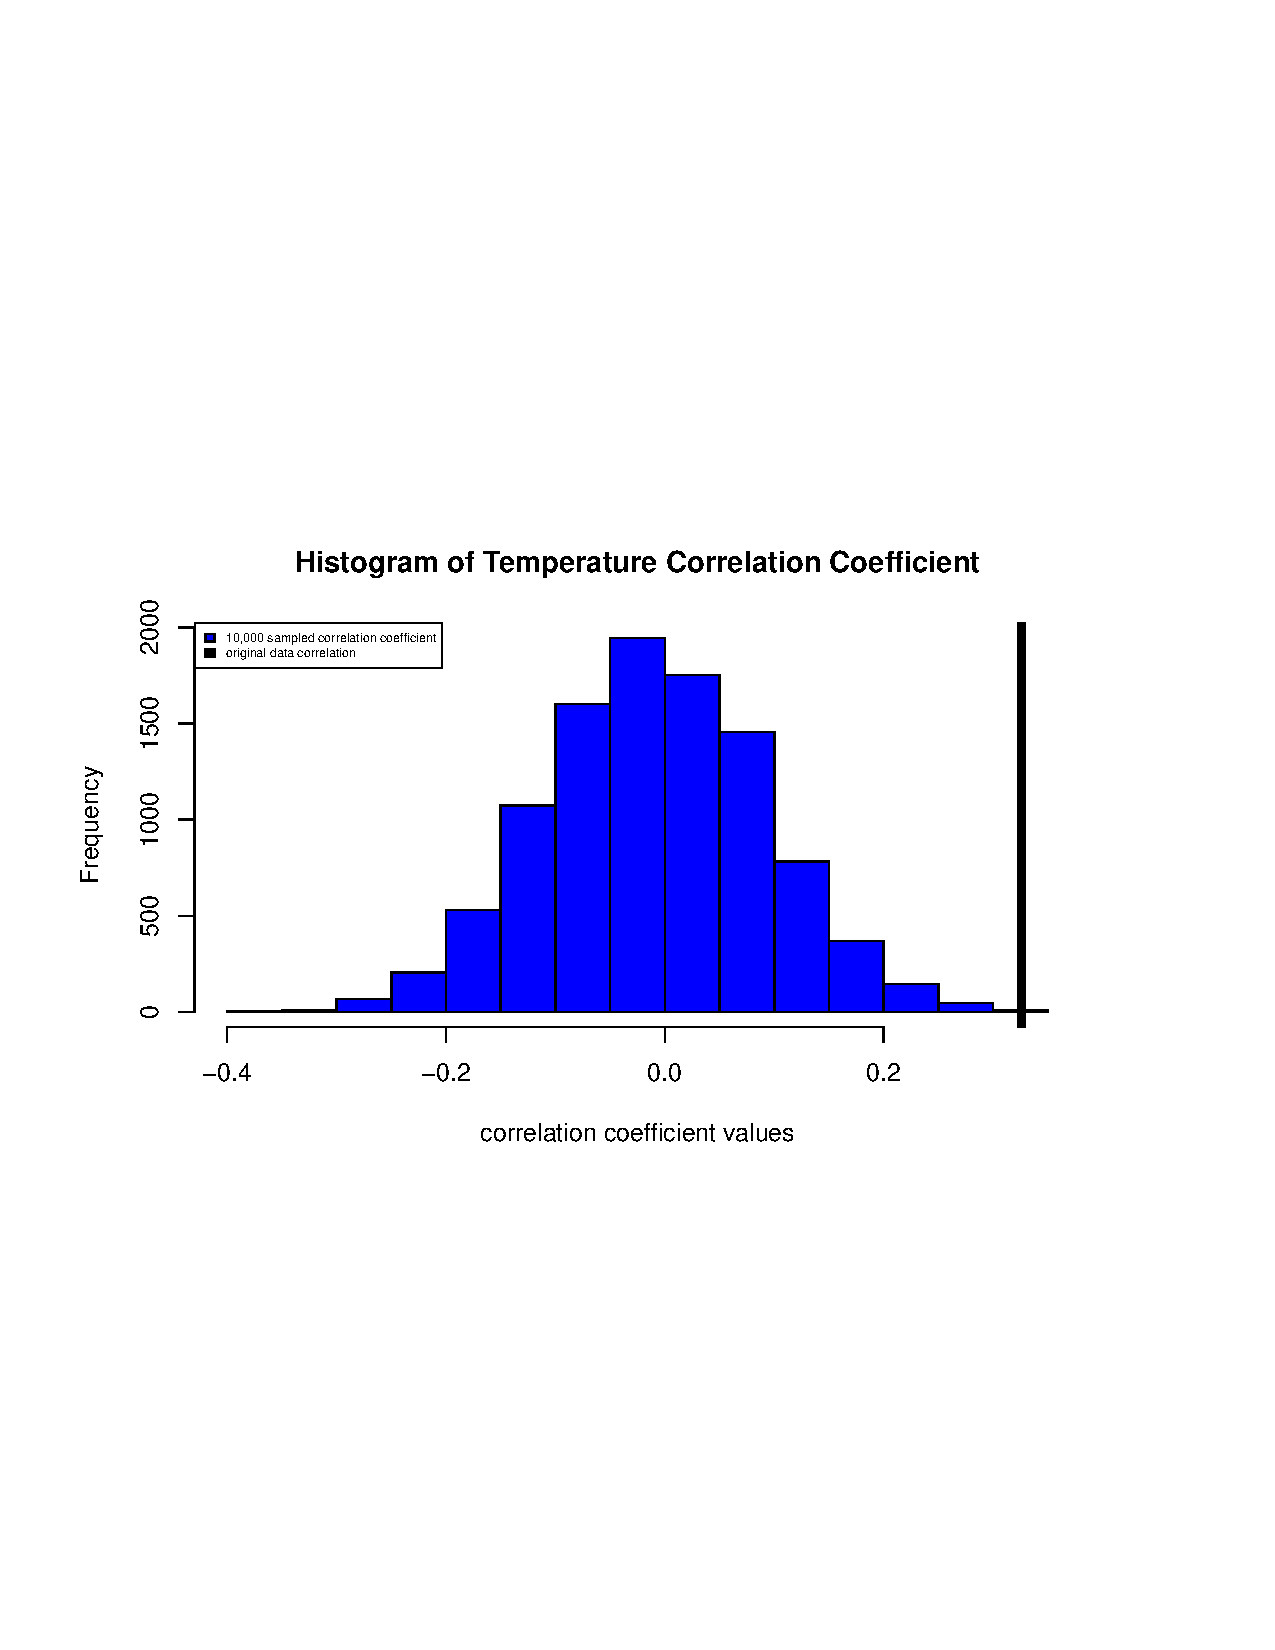
\includegraphics[width=1.2\textwidth]{../Results/TAAutoCorrRplot.pdf}
                \centering
    \end{figure}


\end{document}
